\documentclass[11pt,letterpaper]{article}
\usepackage[utf8]{inputenc}
\usepackage{amsmath,amssymb,fullpage,graphicx}

\let\hat\widehat
\let\tilde\widetilde

\begin{document}
\section*{HW1}
\subsection*{lab0}
\begin{verbatim}
(57/276)^2 + 4.3*0.001 ## 0.04695123

x = 3
x ## 3
y = 1 + 1
y ## 2
log10(y) ## 0.30103
log2(y) ## 1
sqrt(y) ## 1.414214

is.vector(x) ## TRUE

x = 1:5 
x ## 1 2 3 4 5
y = seq(from=0, to=10, by=2)
y ## 0  2  4  6  8 10
y = c(34, 30, 41, 35, 21)
y ## 34 30 41 35 21

mean(y) ## 32.2
median(y) ## 34
range(y) ## 21 41
range(y)[1] ## 21
range(y)[2] ## 41
min(y) ## 21
max(y) ## 41
length(y) ## 5
sort(y) ## 21 30 34 35 41
sd(y) ## 7.395945

data(cars)
?cars
cars
names(cars) ## "speed" "dist"
dim(cars) ## 50 2
cars$speed
cars[, 1]
x = cars$speed
x
mean(x) ## 15.4
sd(x) ## 5.287644

dat = read.table("https://www.stat.washington.edu/marzban/421/autumn19/hist_dat.txt", header=F)
dat
x = dat[, 1]
x
par(mfrow=c(3, 3))
hist(x, breaks = 2)
hist(x, breaks = 3)
hist(x, breaks = 4)
hist(x, breaks = 5)
hist(x, breaks = 10)
hist(x, breaks = 20)
hist(x, breaks = 30)
hist(x, breaks = 100)
hist(x, breaks = 10000)

hist(x, breaks = seq(-3, 7, by=1))

setwd("/Users/nantang/Google Drive/STAT 421/HW/HW1/")
pdf("hello.pdf")
par(mfrow=c(1,2))
hist(x)
hist(x, freq=F)
dev.off()

dbinom(0, 100, 0.005) ## 0.6057704
dbinom(0:3, 100, 0.005) ## 0.60577044 0.30440725 0.07571939 0.01242965
sum(dbinom(0:3, 100, 0.005)) ## 0.9983267
plot(0:3, dbinom(0:3, 100, 0.005))

x = 0:10
plot(x, dpois(x, 1), type="b")
lines(x, dpois(x, 4), type="b", col=2)
lines(x, dpois(x, 6), type="b", col=3)

x = 0:100
plot(x, dnorm(x, 40, 10))

rbinom(200, 10, 0.5)
rpois(100, 4)
x = rnorm(10000, 0, 1)
hist(x, breaks=200)

boxplot(x, range=0)
boxplot(x, x)

quantile(x, prob=c(0, 0.25, 0.5, 0.75, 1))

x = rnorm(500, 0, 1)
hist(x)
qqnorm(x)

x = rexp(500, 1)
hist(x)
qqnorm(x)

library(lattice)
x = rexp(500, 1)
hist(x)
qqmath(x, dist=qexp)
\end{verbatim}

\section*{HW2}
\subsection*{1.9}
Q: Why randomization important in an experiment?
\begin{itemize}
\item Many statistical methods base on the assumption that observations are independently distributed random variables whose possible possible outcomes are of random phenomenon. Randomization ensures both allocation of experimental material and the order are randomly determined, therefore make the random variable assumption usually valid. 
\item By randomization, we can average out unexpected and uninterested effects from extraneous factors. The uninterested effects may introduce systematic bias into experiment results without randomly allocating experiment materials. 
\end{itemize}

\subsection*{Lect 2-1}
\subsection*{a}
In paired design, we may look at differences in number within each pair. \\
If we consider tip as the only treatment factor, replication as a factor, then such design is looking for the differences within pairs $(Y_{111}, Y_{211})$, $(Y_{112}, Y_{212})$, $(Y_{121}, Y_{221})$, $(Y_{221}, Y_{222})$.

\subsection*{b}
Since replication is supposed to be non effective, and coupon is a blocking factor, we are interested in difference in means for two separate blocks.
They are difference between $\frac{Y_{111} + Y_{112}}{2}$ and $\frac{Y_{211} + Y_{212}}{2}$, and difference between $\frac{Y_{121} + Y_{122}}{2}$ and $\frac{Y_{221} + Y_{222}}{2}$

\subsection*{c}
$\frac{Y_{111} + Y_{112}}{2} = Y_{11.} / 2$ \\
$\frac{Y_{211} + Y_{212}}{2} = Y_{21.} / 2$\\
$\frac{Y_{121} + Y_{122}}{2} = Y_{12.} / 2$ \\
$\frac{Y_{221} + Y_{222}}{2} = Y_{22.} / 2$\\

\subsection*{Lect 2-2}
\begin{verbatim}
m1 <- c(0.73, 0.62, 0.62, 0.82, 0.68)
m2 <- c(0.75, 0.55, 0.64, 0.00, 0.30)
m3 <- c(0.65, 0.46, 0.52, 0.48, 0.64)
m4 <- c(0.71, 0.49, 0.56, 0.66, 0.99)
m5 <- c(0.61, 0.28, 0.35, 0.62, 0.52)
m6 <- c(0.75, 0.34, 0.89, 0.66, 0.80)
m7 <- c(0.08, 0.27, 0.28, 0.49, 0.81)
m8 <- c(0.87, 0.97, 0.78, 0.98, 0.75)

all_m <- list(m1,m2,m3,m4,m5,m6,m7,m8)

boxplot(all_m, range=0, xlab="Model Type", ylab="Accuracy")
\end{verbatim}

\includegraphics[scale=0.45]{lec-2-2.png}

\begin{itemize}
\item If we focus on the median, model 8 has highest median accuracy, model 7 has lowest median accuracy. 
\item if we focus on the range, model 2 and model 7 have largest range of accuracy, model 1 and model 3 have narrowest. The spread of accuracy in model 8 is also relatively narrow. 
\item If we focus on the inter-quartile range, model 1 has smallest box, model eight has largest box. Meanwhile, model 3, 4, and 6 have relatively small inter-quartile range. 
\item Overall, model 8 has relatively narrow spread of accuracy and highest median, implying this model may perform stable and precise prediction. Model 2 has largest inter-quartile range and lowest lower whisker, indicating such model perform unstably. Model 7 has lowest median, indicating half of its runs have low accuracy. 
\item Since other models have large proportion of overlap, and each model has only five replications, it is hard to determine if difference exists between these models. 
\end{itemize}

\subsection*{Lect 2-3}
\subsection*{a}
Possible sample geometric means are $1$, $\sqrt{2}$, $\sqrt{3}$, $2$, $\sqrt{6}$, $3$\\
\begin{align*}
P(1) &= P(1, 1) =  \frac{1}{2} \cdot \frac{1}{2} = \frac{1}{4} \\
P(\sqrt{2}) &= P(2, 1) \text{ or } P(1,2)=  \frac{1}{2} \cdot \frac{1}{4} \cdot 2 = \frac{1}{4} \\
P(\sqrt{3}) &= P(3,1) \text{ or } P(1,3) = \frac{1}{4} \\
P(2) &= P(2, 2) = \frac{1}{16} \\
P(\sqrt{6}) &= P(2, 3) \text{ or } P(3, 3) = \frac{1}{8} \\
P(3) &= P(3,3) =  \frac{1}{16}
\end{align*}

\subsection*{b}
\begin{verbatim}
trial <- 1000
x <- c(1, 2, 3)
x_prob <- c(1/2, 1/4, 1/4)
geo_mean <- numeric(1000)
for (i in 1:trial) {
  samp <- sample(x, size=2, prob = x_prob, replace=T)
  geo_mean[i] = sqrt(samp[1] * samp[2])
}
geo_mean_prob <- as.vector(table(geo_mean)) / trial
x_val <- c(1, sqrt(2), sqrt(3), 2, sqrt(6), 3)

plot(x_val, geo_mean_prob, type='h', lwd=5, xlab='Geometric Means', ylab='Density',
     main='Sampling Distribution')
\end{verbatim}
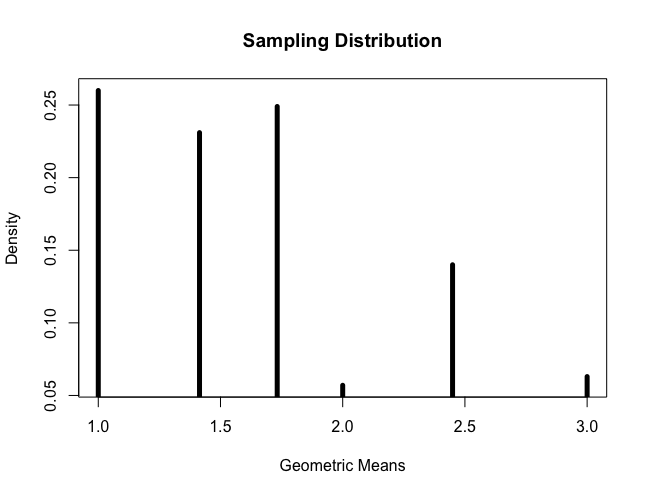
\includegraphics[scale=0.45]{lec-2-3-b.png}

\subsection*{c}
\begin{verbatim}
x_val <- c(1, sqrt(2), sqrt(3), 2, sqrt(6), 3)
y_val <- c(1/4, 1/4, 1/4, 1/16, 1/8, 1/16)
plot(x_val, geo_mean_prob, type='h', lwd=5, xlab='Geometric Means', ylab='Density',
     main='Sampling Distribution')
points(x_val, y_val, cex=2, pch=20, col=2)

\end{verbatim}
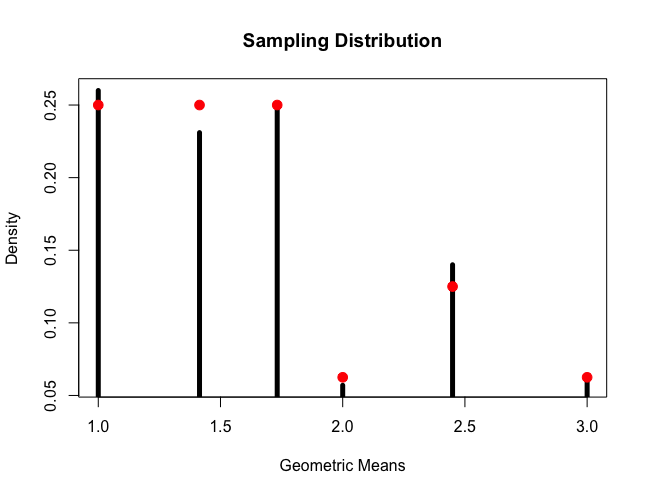
\includegraphics[scale=0.5]{lec-2-3-c.png}

\end{document}